\documentclass[a4paper,english]{scrreprt}

% Uncomment to optimize for double-sided printing.
% \KOMAoptions{twoside}

% Set binding correction manually, if known.
% \KOMAoptions{BCOR=2cm}

% Localization options
\usepackage[german]{babel}
\usepackage[T1]{fontenc}
\usepackage[utf8]{inputenc}

% Enhanced verbatim sections. We're mainly interested in
% \verbatiminput though.
\usepackage{verbatim}

% PDF-compatible landscape mode.
% Makes PDF viewers show the page rotated by 90°.
\usepackage{pdflscape}

% Advanced tables
\usepackage{tabu}
\usepackage{longtable}
\usepackage{dcolumn}
\newcolumntype{d}[1]{D{.}{\cdot}{#1} }

% Fancy tablerules
\usepackage{booktabs}

% Graphics
\usepackage{graphicx}

% Current time
\usepackage[useregional=numeric]{datetime2}

% Float barriers.
% Automatically add a FloatBarrier to each \section
\usepackage[section]{placeins}

% Custom header and footer
\usepackage{fancyhdr}

\usepackage{geometry}
\usepackage{layout}

% Math tools
\usepackage{mathtools}
% Math symbols
\usepackage{amsmath,amsfonts,amssymb}
\usepackage{amsthm}

% SI units
\usepackage{siunitx}
\DeclareSIUnit\Molar{\textsc{m}}
\DeclareSIUnit\mole{mol}
\DeclareSIUnit\rpm{rpm}
\DeclareSIUnit\cfu{cfu}

% Chemistry
\usepackage{mhchem}

% Subfigures & captions
\usepackage{subcaption}
\usepackage{wrapfig}

\DeclarePairedDelimiter\abs{\lvert}{\rvert}

\pagestyle{plain}
% \fancyhf{}
% \lhead{}
% \lfoot{}
% \rfoot{}
% 
% Source code & highlighting
\usepackage{listings}

% Convenience commands
\newcommand{\mailsubject}{2027 - Lab course biochemistry 1}
\newcommand{\maillink}[1]{\href{mailto:#1?subject=\mailsubject}
                               {#1}}

% Should use this command wherever the print date is mentioned.
\newcommand{\printdate}{\today}

\subject{2027 - Lab course biochemistry 1}

\title{11 - Isolierung und Charakterisierung von Membranlipiden}

\author{Michael Senn \maillink{michael.senn@students.unibe.ch} - 16-126-880 - Gruppe 14}

\date{\printdate}

% Needs to be the last command in the preamble, for one reason or
% another. 
\usepackage{hyperref}


\begin{document}
\maketitle

\chapter{Einleitung}

Zwecks Kompartmentalisierung zwischen wie auch innerhalb der Zelle finden sich
in vielen Organismen Membrane. Diese sind selektiv durchlässig für verschiedene
metabolische Produkte, und dienen dem kontrollierten Informationsaustausch
zwischen Zellen. Ein wichtiger Bestandteil dieser Membrane sind Membranlipide.
Eine deren Klasse - die Phospholipide - wurde in diesem Versuch genauer
untersucht.

\section{Phospholipide}

Phospholipide bestehen im Allgemeinen aus zwei hydrophoben Fettsäuren, und
einem hydrophilen Kopf bestehend aus einer Phosphat-Gruppe, verbunden mittels
einem Glycerol. Dies erlaubt in wässrigem Medium die Bildung einer
Doppellipidschicht, in welcher die Fettsäuren gegen innen, und die
Phosphat-Gruppen gegen aussen zeigen.

Durch Anlagerung verschiedener organischer Moleküle an der Phosphatgruppe
ergeben sich Klassen von Phospholipiden mit unterschiedlich polaren
Kopfgruppen.

\subsection{Polarität der Kopfgruppen}

Für vier dieser Klassen soll hier die Polarität der Kopfgruppe hergeleitet
werden. Dies sind Phosphatidylserine (PS), Phosphatidylcholine (PC),
Phosphatidylethanolamine (PE), und Phosphatidylinositol (PI).

\begin{figure}
	\centering
	\includegraphics[width=0.9\textwidth]{img/phospholipide.png}
	\caption{Struktur von vier Klassen von Phospholipiden, aus \cite{handoutv11}}
	\label{fig:phospholipide}
\end{figure}

Phosphatidylcholine mit einem tertiären Amin besitzt die polarste Kopfgruppe
dieser vier Klassen, da eine Verminderung der Ladung aufgrund der stabilen
\ce{CH3} Reste kaum möglich ist.

Phosphatidylethanolamin hat Aufgrund der in Abbildung \ref{fig:phospholipide}
ersichtlichen positiv geladenen Amino-Gruppe die am zweitstärksten polare
Kopfgruppe. Da es sich hierbei aber um ein primäres Amin handelt, kann diese
Ladung durch Deprotonierung neutralisiert werden.

Phosphatidylserin hat, in dem im Versuch verwendeten Lösungsmittel Chloroform,
nur eine schwache Ladung auf der Carboxylgruppe, und somit den drittpolarsten
Kopf.

Phosphatidylcholine besitzt ein, in Abbildung \ref{fig:phospholipide}
sichtbares, Ringsystem. Dessen elektronenstabilisiernde Eigenschaft führt dazu,
dass PC die am wenigsten polare Kopfgruppe besitzt.

\subsection{Einfluss der Fettsäuren auf auf Membranrigidität}

Der Aufbau der Fettsäuren beeinflusst die Rigidität der Membrane auf zwei Arten.
Längere Fettsäuren führen, aufgrund stärkerer Van-der-Waals-Kräfte, zu einer
rigideren Membran. Ungesättigte Fettsäuren - das heisst Fettsäuren mit C-C
Doppelbindungen - besitzen einen Knick welcher dazu führt dass die Fettsäuren
weniger dicht gepackt sind, was zu einer weniger rigiden Membran führt

\section{Chromatographie}

Die Chromatographie nutzt Interaktionen zwischen Molekülen dazu, ein Gemisch
basierend auf einer oder mehreren Eigenschaften aufzutrennen. Allen
Chromatographiemethoden ist gemein dass zwei Phasen verwendet werden - die
mobile Phase in welcher das aufzutrennende Gemisch wandert, und die stationäre
Phase, deren Wechselwirkungen mit dem Gemisch bestimmen wie schnell die
einzelnen Komponenten wandern.

Je nach Aufbau der stationären Phase kann beispielsweise nach Ladung oder
Grösse aufgetrennt werden. In unserem Versuch wurden zwei Arten der
Chromatographie verwendet - die Dünnschichtchromatographie und die
Gaschromatographie.

\subsection{Dünnschichtchromatographie}

In der Dünnschichtchromatographie wurde ein apolares Lösungsmittel als mobile
Phase, und ein polares Silicagel als stationäre Phase verwendet. Phospholipide
mit polaren Kopfgruppen interagierten stärker mit der stationären Phase als
jene mit apolaren Kopfgruppen, wodurch eine Auftrennung nach Polarität der
Kopfgruppe stattfand - je apolarer die Kopfgruppe, umso weiter wanderten die
Lipide auf der stationären Phase.

Zwecks Analyse der aufgetrennten Phospholipiden wurden die Versuchsreihen mit
Farbstoffen eingefärbt. Dichlorofluoreszin zwecks Detektion von Lipiden,
Ninhydrin zwecks Detektion von freien Aminen, und Molybdän zwecks Detektion
von Phosphatgruppen.

\subsection{Gaschromatographie}

In der Gaschromatographie wurde als stationäre Phase ein inertes Gas verwendet,
welches durch eine Säule - ein langer dünner Schlauch - floss. Als stationäre
Phase diente Quarzglas, mit welchem das Innere der Säule ausgekleidet war.

Die aufzutrennenden Phospholipide wurden durch langsames erhöhen der Temperatur
in die Gasphase überführt, wobei jene mit polaren Kopfgruppen aufgrund stärkerer
Interaktion mit der stationären Phase erst bei höheren Temperaturen in die
Gasphase übergingen.

Zur Detektion der Moleküle in der Gasphase diente ein
Flammenionisationsdetektor am Ende der Säule, zusammen mit einer
bereitgestellten Messreihe einer Referenzlösung von verschiedenen
Phospholipiden.

\section{Transesterifizierung}

Da die Gaschromatographie nur mit flüchtigen Stoffen funktioniert, wurden die
Phospholipide vorgängig mittels Transesterifizierung zu Fettsäuremethylestern
überführt. \cite{handoutv11}

Hierbei wird durch Zugabe eines Überschusses an Methanolat, und Heizen auf
\SI{75}{\celsius} für \SI{7}{\min} die endotherme Reaktion in Richtung der
Fettsäuremethylester bevorzugt. Die Reaktion wird durch Zugabe von \ce{KH2PO4}
abgebrochen, welches die überschüssigen freien Methanolate protoniert.

Der Reaktionsmechanismus ist in Abbildung \ref{fig:transesterifizierung}
zusammengefasst.

\begin{figure}
	\centering
	\includegraphics[width=0.3\textwidth]{img/transesterifizierung.png}
	\caption{Transesterifizierung von Phospholipiden, aus \cite{handoutv11}}
	\label{fig:transesterifizierung}
\end{figure}

Durch Zugabe von Hexan lassen sich die vergleichsweise apolaren
Fettsäuremethylester extrahieren und für die Gaschromatographie verwenden.

\section{Ziel}

Ziel des Experimentes war es, die Zusammensetzung der Lipiden in E. coli
Membranen bei unterschiedlichen Temperaturen zu untersuchen. Hierzu wurden
Lipide aus E. coli Kulturen welche bei \SI{20}{\celsius} respektive
\SI{37}{\celsius} gezüchtet wurden extrahiert, und mittels Chromatographie
aufgetrennt und analysiert.

\subsection{Hypothesen}

Drei Hypothesen wurden aufgestellt:
\begin{enumerate}
	\item In der \SI{20}{\celsius} Kultur sind Fettsäuren durchschnittlich
		kürzer als in der \SI{37}{\celsius} Kultur
	\item In der \SI{20}{\celsius} Kultur hat es mehr ungesättigte
		Fettsäuren als in der \SI{37}{\celsius} Kultur
	\item Die polaren Kopfgruppen unterscheiden sich nicht zwischen den
		beiden Kulturen.
\end{enumerate}

\chapter{Durchführung}

Der Versuch wurde gemäss bereitgestelltem Protokoll \cite{skriptv11}
durchgeführt. Abweichungen, Beobachtungen und Messwerte sind hier dokumentiert.

\section{Massebestimmung der isolierten Lipide}

\subsection{Isolation der Membranlipide}

Bei Zugabe des heissen Methanols bildete sich ein Ausfall. Dieser Ausfall
enthielt alle Zellbestandteile welche nicht im apolaren Methanol lösbar waren -
beispielsweise polare Proteinn, oder die negativ geladene DNA.

Nach der Abdestillation des Methanols wurden die Lipidrückstände versehentlich
mit reinem \ce{CH3Cl} anstelle einer 1:1 Mischung aus \ce{CH3Cl} und \ce{MeOH}
gelöst und durch den Baumwollfilter gelassen. Zur Korrektur wurden die
Rückstände im Rundkolben ein weiteres Mal mit \SI{1}{\ml} 1:1
\ce{CH3Cl}:\ce{MeOH} gelöst, und diese Lösung ebenfalls durch den
Baumwollfilter gegeben. Das zweite Nachspülen mit 1:1 \ce{CH3Cl}:\ce{MeOH} fand
gemäss Protokoll statt.

Bei der Zugabe der Lösungsmittels wurde eine leichte Verfärbung beobachtet, was
impliziert dass sich gewisse Bestandteile des Rückstandes lösten.

\subsection{Bestimmung der isolierten Lipidmenge}

Da die Analysewaage defekt war, musste die Messung mit der Oberschalenwaage
durchgeführt werden. Aufgrund deren fehlenden Genauigkeit konnte die isolierte
Menge nicht bestimmt werden, und die Menge von isolierten Lipiden wurde von
Auge geschätzt. Alle unsere Proben wurden in \SI{1}{\ml} \ce{CHCl3} gelöst, die
gewünschte Endkonzentration von \SI{20}{\mg\per\ml} war damit nur approximativ
möglich.

\section{Dünnschichtchromatographie}

Die DC Platte wurde gemäss Ladeschema in Tabelle \ref{tbl:dc_ladeschema} mit
den extrahierten Lipiden der beiden Kulturen, und einer Referenzlösung,
bestückt.

\begin{table}
	\centering
	\begin{tabu}{l|ccc|c|ccc|c|ccc|c}
		\toprule
		                  & 1 & 2 & 3 & 4 & 5 & 6 & 7 & 8 & 9 & 10 & 11 & 12 \\
		\midrule
		\SI{20}{\celsius} & x &   &   &   & x &   &   &   & x &    &    &    \\
		\SI{37}{\celsius} &   & x &   &   &   & x &   &   &   & x  &    &    \\
		Referenz          &   &   & x &   &   &   & x &   &   &    & x  &    \\
		\midrule
		Farbstoff         & \multicolumn{3}{c|}{Dichlorof.} & & \multicolumn{3}{c|}{Ninhydrin} & & \multicolumn{3}{c|}{Molybdän} \\
		\bottomrule
	\end{tabu}
	\caption{Ladeschema für Dünnschichtchromatographie}
	\label{tbl:dc_ladeschema}
\end{table}

Die Resultate der Dünnschichtchromatographie werden in der Auswertung besprochen.

\chapter{Auswertung DC}

\section{Resultate}

In Abbildung \ref{fig:dc_resultat} sind die beschrifteten Resultate der
Dünnschichtchromatographie dargestellt. Auf die Gruppen von Flecken A bis G
soll hier eingegangen werden.

\subsection{Bedeutung der Färbungen}

Eine Einfärbung mit Dichlorofluoreszin impliziert, dass es sich bei der
fraglichen Probe um ein Lipid handelt. Ninhydrin bindet an freie Amingruppen,
und Molybdän an Phosphatgruppen.

\subsection{A: Phosphatidylethanolamin}

Aus den Färbungen ist ersichtlich, dass es sich um ein Lipid, mit freiem Amin,
und einer Phosphatgruppe handelt. Zusammen mit der aus der Laufhöhe
ersichtlichen mittleren Polarität muss es sich hierbei um PE handeln.

\subsection{B: Phosphatidylcholin}

Gemäss den Färbungen handelt es sich um ein Phospholipid ohne freies Amin, das
zudem aufgrund tieferer Laufhöhe polarer als PE ist. Dies impliziert dass es
sich um PC handelt.

\subsection{C: Phosphatidylserin}

Hierbei handelt es sich ebenfalls um ein Phospholipid ohne freies Amin, welches
aber weniger polar als PE ist. Folglich handelt es sich hierbei um PS.

\subsection{D: Phosphatidylinositol}

Dieses Lipid das fast auf Höhe der Laufmittelfront ist ist folglich sehr
apolar, deshalb muss dies PI sein. Erwartet wäre aufgrund der Phosphatgruppe
eine Färbung der Molybdänbande gewesen, jener Farbstoff bedingt aber eine hohe
Konzentration Substrat um sichtbar zu sein, was unter anderem aufgrund der
Ungenauigkeit der Verdünnung nicht gewährleistet war.

\subsection{E: Stark apolare Stoffe}

Bei diesen komplett apolaren Lipiden ohne Phosphatgruppe wird es sich
beispielsweise um freie Fettsäuren oder Triacylglyceride, welche allesamt keine
polaren Kopfgruppen besitzen, handeln.

\subsection{F: Stark polare Stoffe}

Aufgrund der Laufhöhe ist klar dass es sich um stark polare, Amin-haltige,
Stoffe handelt, welche keine Lipide sind. Dies sind Proteine und Aminosäuren,
welche bei der Aufreinigung nicht komplett entfernt wurden.

\subsection{G: Unbekanntes Phospholipid}

Hierbei scheint es sich um ein Phospholipid ohne freies Amin zu handeln,
welches allerdings in der Referenzlösung nicht vorhanden ist, und somit nicht
klassifiziert werden kann.

\begin{figure}
	\centering
	\includegraphics[width=0.9\textwidth]{img/dc_resultat.png}
	\caption{Resultat der Dünnschichtchromatographie, Ladeschema \& Einfärbung gemäss Tabelle \ref{tbl:dc_ladeschema}, Silicagel \& \ce{CH3Cl}}
	\label{fig:dc_resultat}
\end{figure}

\section{Interpretation}

Von den vier untersuchten Phospholipiden sind in E. coli Zellen nur PE und PC
vorhanden. Weiterhin sind beide dieser Phospholipide sowohl in der
\SI{20}{\celsius} als auch in der \SI{37}{\celsius} Probe enthalten. Die
Abwesenheit von PC in der Dichlorofluoreszin-Färbung der \SI{37}{\celsius}
Probe lässt sich mit der Ungenauigkeit der Verdünnung erklären - so ist in der
Molybdän-Färbung ein Fleck auf erwarteter Höhe sichtbar.

Qualitativ kann aufgrund der Ungenauigkeit der Verdünnung ohnehin keine Aussage
gemacht werden.

Damit kann die Hypothese, dass sich die polaren Kopfgruppen zwischen den beiden
Kulturen nicht unterscheiden, bestätigt werden.

\chapter{Auswertung GC}

\section{Rohdaten}

\begin{figure}
	\centering
	\begin{subfigure}{.45\textwidth}
		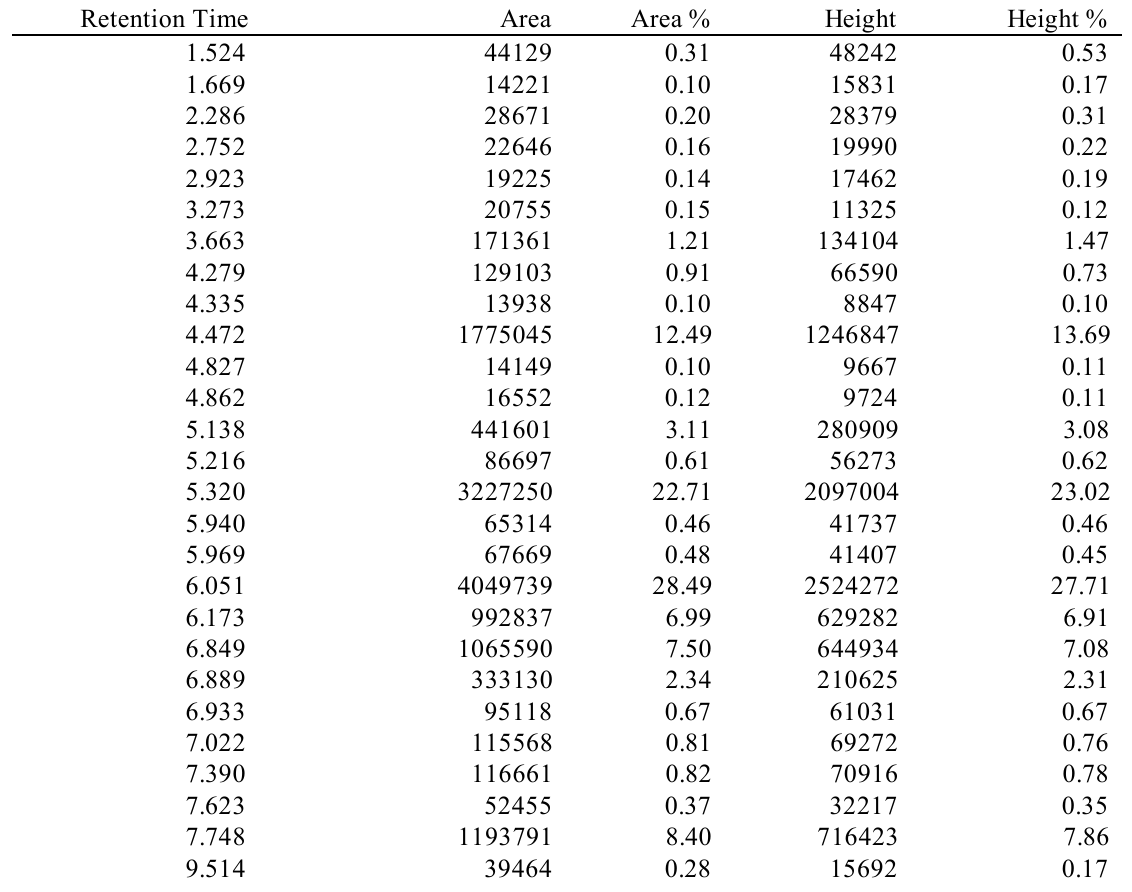
\includegraphics[width=\linewidth]{img/gc_37_roh.png}
		\caption{\SI{37}{\celsius} Kultur}
		\label{fig:gc_37_roh}
	\end{subfigure}
	~
	\begin{subfigure}{.45\textwidth}
		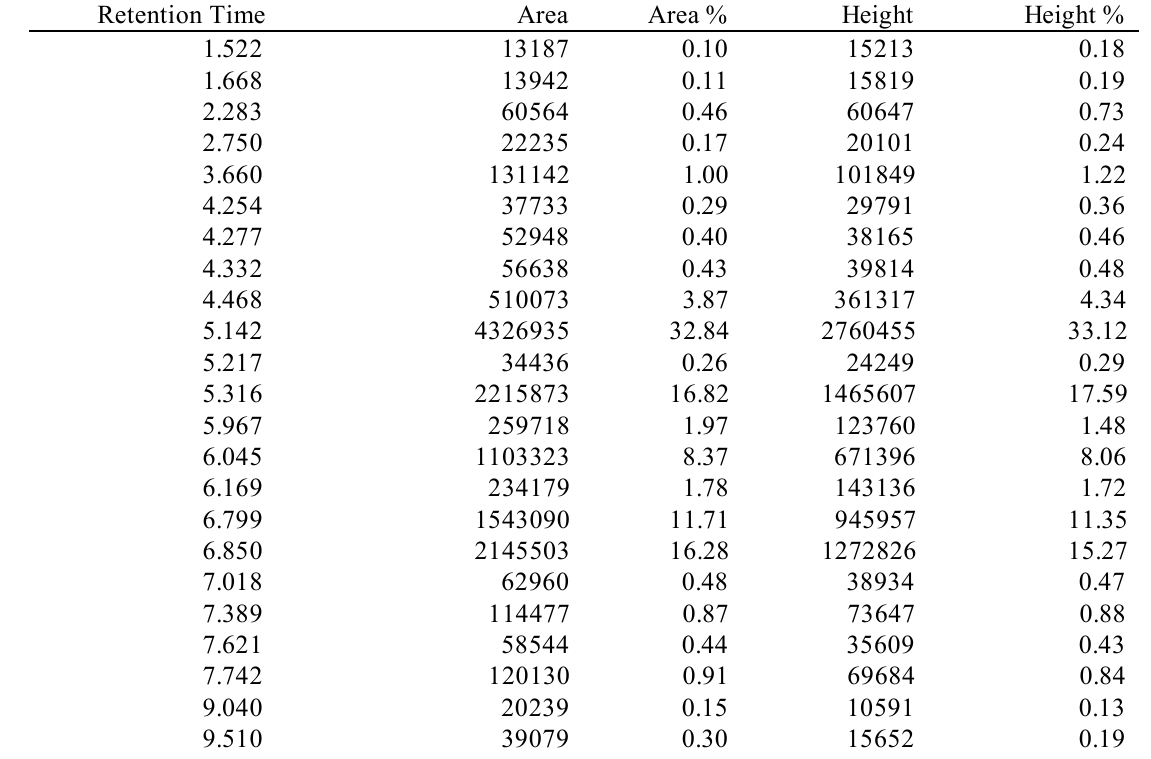
\includegraphics[width=\linewidth]{img/gc_20_roh.png}
		\caption{\SI{20}{\celsius} Kultur}
		\label{fig:gc_20_roh}
	\end{subfigure}
	\caption{Rohdaten der Gaschromatographie}
	\label{fig:gc_roh}
\end{figure}

\begin{figure}
	\centering
	\begin{subfigure}{\textwidth}
		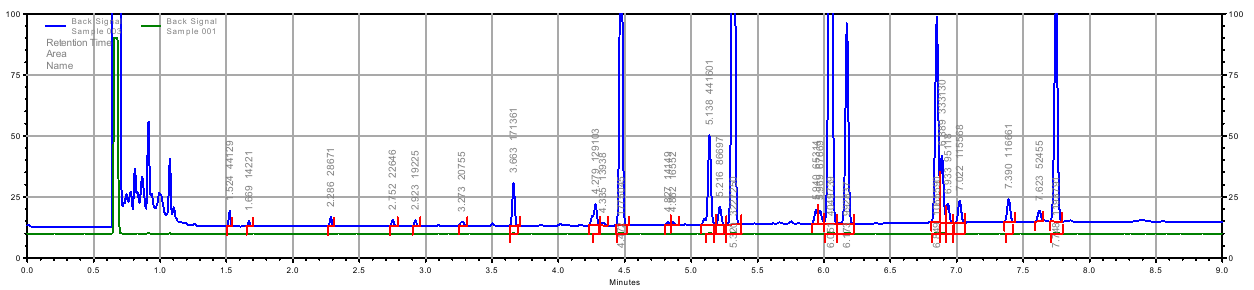
\includegraphics[width=\linewidth]{img/gc_37_chromatogramm.png}
		\caption{\SI{37}{\celsius} Kultur}
		\label{fig:gc_37_chromatogramm}
	\end{subfigure}
	\begin{subfigure}{\textwidth}
		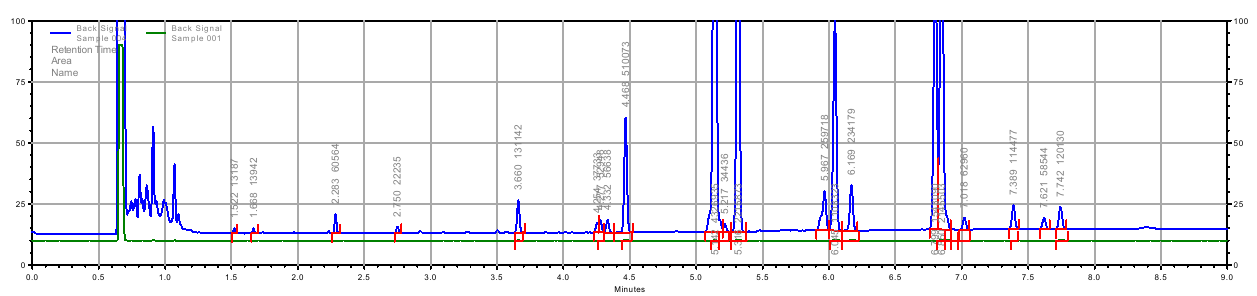
\includegraphics[width=\linewidth]{img/gc_20_chromatogramm.png}
		\caption{\SI{20}{\celsius} Kultur}
		\label{fig:gc_20_chromatogramm}
	\end{subfigure}
	\caption{Automatisch erstelltes Chromatogramm der Gaschromatographie}
	\label{fig:gc_chromatogramm}
\end{figure}


In Abbildung \ref{fig:gc_37_roh} sind die GC-Rohdaten der \SI{37}{\celsius}
Kultur, in Abbildung \ref{fig:gc_20_roh} jene der \SI{20}{\celsius} Kultur
dargestellt. Entsprechend finden sich in Abbildung \ref{fig:gc_chromatogramm}
die automatisch erstellen Chromatogramme für die beiden Kulturen. Die grossen
Peaks auf der linken Seite entsprechen dabei dem verwendeten Lösungsmittel.

\subsection{Verteilung der detektierten Stoffen}

Direkt ist ersichtlich, dass die Mehrheit der Peaks der beiden Chromatogramme in
Abbildung \ref{fig:gc_chromatogramm} an der gleichen Stelle sind. Dies
impliziert, dass bei beiden Kulturen mehrheitlich die gleichen Membranlipide
ausgebildet werden. Die \SI{37}{\celsius} Kultur scheint aber ein marginal
breiteres Spektrum zu haben, bei welchem gewisse Stoffe zusätzlich, oder in
grösserer Konzentration, gebildet werden als in der \SI{20}{\celsius} Kultur.

\section{Zuordnung der stärksten Signale zu Fettsäuren}

Alle Stoffe, die in wenigstens einer der beiden Gaschromatographien einen
Flächenanteil von mindestens \SI{5}{\percent} besassen, wurden in eine separate
Tabelle extrahiert und mittels bereitgestellter Referenztabelle den Fettsäuren
zugeordnet. Die Resultate dieser Zuordnung finden sich in Tabelle
\ref{tbl:gc_fs_haeufig}.

\begin{table}
	\centering
	\begin{tabu}{lllll}
		\toprule
		Fettsäure (C:D) & \multicolumn{2}{c}{Retention time [\si{\s}]} & \multicolumn{2}{c}{Area [\si{\percent}]} \\
		                & \SI{20}{\celsius} & \SI{37}{\celsius}  & \SI{20}{\celsius} & \SI{37}{\celsius} \\
		\midrule
		15:0           & 4.468 & 4.472 & 3.87  & 12.49 \\
		16:$1^9$       & 5.142 & 5.138 & 32.84 & 3.11  \\
		16:0           & 5.316 & 5.32  & 16.82 & 22.71 \\
		17:0$\Delta$   & 6.045 & 6.051 & 8.37  & 28.49 \\
		17:0           & 6.169 & 6.173 & 1.78  & 6.99  \\
		18:$1^9$ trans & 6.799 & 6.802 & 11.71 & 0     \\
		18:$1^9$ cis   & 6.85  & 6.849 & 16.28 & 7.5   \\
		19:0$\Delta$   & 7.742 & 7.748 & 0.91  & 8.4   \\
		\bottomrule
	\end{tabu}
	\caption{Zuordnung von Fettsäuren mit mindestens \SI{5}{\percent}}
	\label{tbl:gc_fs_haeufig}
\end{table}

\subsection{Auswertung}

Die Daten aus Tabelle \ref{tbl:gc_fs_haeufig} wurden mittels Balkendiagramm in
Abbildung \ref{fig:gc_fs_haeufig} visualisiert. Es ist sofort ersichtlich, dass
alle gesättigten Fettsäuren (15:0, 16:0, 17:0, 17:0$\Delta$, 19:0$\Delta$) in
der \SI{37}{\celsius} Kultur viel häufiger vorkommen als in der
\SI{20}{\celsius} Kultur. Analog sind alle ungesättigten Fettsäuren (16:$1^9$,
18:$1^9$ cis, 18:$1^9$ trans) in der \SI{20}{\celsius} Kultur häufiger
vorhanden.

Weiterhin scheint ein Trend zu bestehen, dass der Konzentrations-Peak der
\SI{20}{\celsius} Kultur bei kürzeren Fettsäuren liegt als jener der
\SI{37}{\celsius} Kultur, was nachfolgend genauer untersucht wird.

Bereits jetzt lässt sich aber die Hypothese, dass die Membran bei tieferen
Temperaturen mehr ungesättigte Fettsäuren enthält, bestätigen.

\begin{figure}
	\centering
	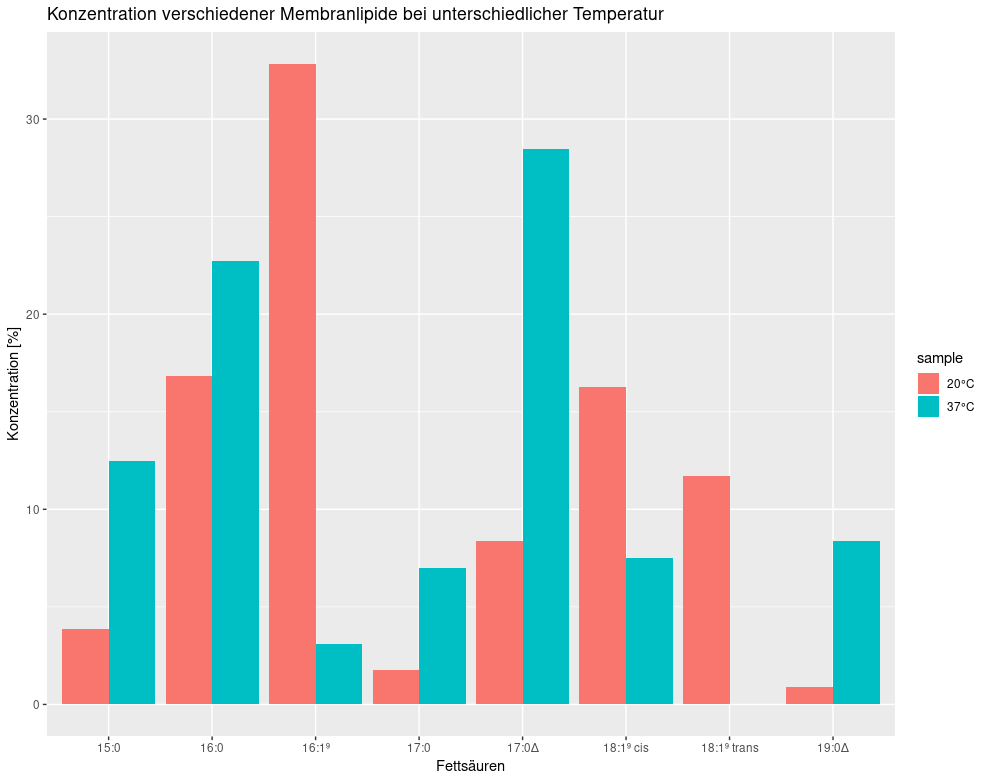
\includegraphics[width=\textwidth]{img/gc_membranlipide.png}
	\caption{Vergleich der Konzentration häufiger Membranlipide bei \SI{20}{\celsius} und \SI{37}{\celsius}}
	\label{fig:gc_fs_haeufig}
\end{figure}

\section{Vergleich der Fettsäurenlänge}

Basierend auf den Rohdaten aus Abbildung \ref{fig:gc_roh} wurden alle möglichen
Fettsäuren zugeordnet, und deren Grösse, als Länge der C-Kette, bestimmt. Diese
Resultate finden sich in Tabelle \ref{tbl:gc_fs_laenge}

\begin{table}
	\begin{tabu}{lllll}
		\toprule
		Fettsäure (C:D) & Retention time [\si{\s}] & Area [\si{\percent}] & Kultur             & Länge (C-Kette) \\
		\midrule
		12:0            &  2.283                   &  0.46                &  \SI{20}{\celsius} &  12 \\
		14:0            &  3.66                    &  1                   &  \SI{20}{\celsius} &  14 \\
		15:0            &  4.468                   &  3.87                &  \SI{20}{\celsius} &  15 \\
		16:$1^9$        &  5.142                   &  32.84               &  \SI{20}{\celsius} &  16 \\
		16:0            &  5.316                   &  16.82               &  \SI{20}{\celsius} &  16 \\
		17:0$\Delta$    &  6.045                   &  8.37                &  \SI{20}{\celsius} &  17 \\
		17:0            &  6.169                   &  1.78                &  \SI{20}{\celsius} &  17 \\
		18:$1^9$ trans  &  6.799                   &  11.71               &  \SI{20}{\celsius} &  18 \\
		18:$1^9$ cis    &  6.85                    &  16.28               &  \SI{20}{\celsius} &  18 \\
		18:0            &  7.018                   &  0.48                &  \SI{20}{\celsius} &  18 \\
		19:0$\Delta$    &  7.742                   &  0.91                &  \SI{20}{\celsius} &  19 \\
		12:0            &  2.286                   &  0.2                 &  \SI{37}{\celsius} &  12 \\
		13:0            &  2.923                   &  0.14                &  \SI{37}{\celsius} &  13 \\
		14:0            &  3.663                   &  1.21                &  \SI{37}{\celsius} &  14 \\
		15:0            &  4.472                   &  12.49               &  \SI{37}{\celsius} &  15 \\
		30H-14:0        &  4.862                   &  0.12                &  \SI{37}{\celsius} &  14 \\
		16:$1^9$        &  5.138                   &  3.11                &  \SI{37}{\celsius} &  16 \\
		16:0            &  5.32                    &  22.71               &  \SI{37}{\celsius} &  16 \\
		17:0$\Delta$    &  6.051                   &  28.49               &  \SI{37}{\celsius} &  17 \\
		17:0            &  6.173                   &  6.99                &  \SI{37}{\celsius} &  18 \\
		18:$1^9$ trans  &  6.802                   &  0                   &  \SI{37}{\celsius} &  18 \\
		18:$1^9$ cis    &  6.849                   &  7.5                 &  \SI{37}{\celsius} &  18 \\
		18:0            &  7.022                   &  0.81                &  \SI{37}{\celsius} &  18 \\
		19:0$\Delta$    &  7.748                   &  8.4                 &  \SI{37}{\celsius} &  19 \\
		\bottomrule
	\end{tabu}
	\caption{Zuordnung von allen möglichen Fettsäuren}
	\label{tbl:gc_fs_laenge}
\end{table}

\subsection{Auswertung}

Die Daten aus Tabelle \ref{tbl:gc_fs_laenge} wurden dann per Länge der C-Kette
und Kultur summiert, und in einem Scatterplot in Abbildung
\ref{fig:gc_fs_laenge} dargestellt. Zwecks besserer visueller Darstellung wurde
zwischen je zwei benachbarten Datenpunkten eine lineare Approximation
eingefügt.

\begin{figure}
	\centering
	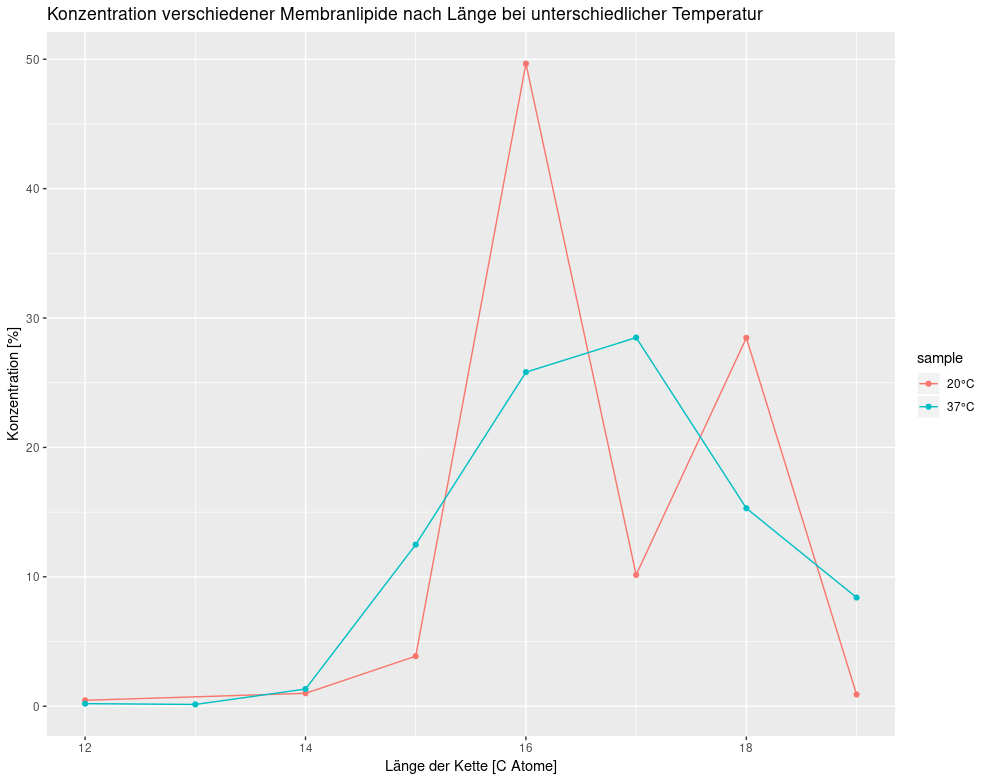
\includegraphics[width=\textwidth]{img/gc_membranlipide_laenge.png}
	\caption{Vergleich der Konzentration verschiedener Membranlipide nach Länge bei \SI{20}{\celsius} und \SI{37}{\celsius}}
	\label{fig:gc_fs_laenge}
\end{figure}

Basierend auf dieser Auswertung kann die Hypothese, dass die Membran bei
tieferen Temperaturen aus kürzeren Fettsäuren besteht, nicht bestätigt werden.
Zwar scheint bei \SI{20}{\celsius} das Konzentrations-Peak bei kürzeren
Fettsäuren zu sein, doch gibt es auch weiterhin viele - bei gewissen Längen
sogar mehr - lange Fettsäuren.

Dies lässt sich mit der nach Konzentration gewichteten durchschnittlichen
Kettenlänge bestätigen - für die \SI{20}{\celsius} Kultur ergibt dies einen
Wert von 16.66 C-Atomen, für die \SI{37}{\celsius} Kultur einen Wert von 16.74.
Dieser Unterschied scheint vernachlässigbar, besonders unter Betrachtung der
Ungenauigkeit des Experimentes.

\chapter{Schlussfolgerungen}

\section{Zusammenfassung}

Zusammenfassend lässt sich sagen:

\begin{itemize}
	\item Es kann nicht bestätigt werden, dass bei tieferen Temperaturen
		die Fettsäuren der Membranlipide kürzer sind. Für eine genauere
		Untersuchung müsste ein Experiment mit höherer Genauigkeit
		durchgeführt werden.
	\item Es kann bestätigt werden, dass bei Tieferen Temperaturen in der
		Membran mehr ungesättigte Fettsäuren vorkommen.
	\item Es kann bestätigt werden, dass die Temperatur keinen Einfluss
		auf die Kopfgruppen der Phospholipide der Membran hat.
\end{itemize}

\section{Reaktionsmechanismus Glycerol-2-Phosphat}

Durch Abspaltung der Fettsäuren in der Transesterifizierung bleibt
Glycerol-1-Phosphat übrig. Durch einen intramolekularen nukleophilen Angriff
des elektronegativen Sauerstoffs auf die Phosphatgruppe kommt es zu einer
Bildung einer Ringstruktur, und durch die Protonierung des Sauerstoffs der
Phosphatgruppe zur Abspaltung der ehemaligen Kopfgruppe des Phospholipides.

Nach anschliessender Ringöffnung bleibt ein Glycerol-2-Phosphat.

Die Kopfgruppe die im Falle der Transesterifizierung der Phospholipide noch
vorhanden ist, kann durch Protonierung des Sauerstoff-Atoms der Phosphatgruppe
abgehen.

\begin{figure}
	\centering
	\begin{subfigure}{.9\textwidth}
		
\includegraphics[width=0.5\linewidth]{img/glycerol_1_phosphat.png}
		\caption{Glycerol-1-Phosphat}
	\end{subfigure}

	\begin{subfigure}{.9\textwidth}
		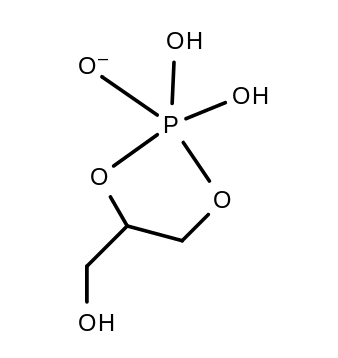
\includegraphics[width=0.5\linewidth]{img/glycerol_phosphat_ring.png}
		\caption{Intermediäre Ringstruktur}
	\end{subfigure}

	\begin{subfigure}{.9\textwidth}
		
\includegraphics[width=0.5\linewidth]{img/glycerol_2_phosphat.png}
		\caption{Glycerol-2-Phosphat}
	\end{subfigure}
\end{figure}



\bibliographystyle{vancouver}
\bibliography{references}

\end{document}
